\documentclass{article}
\usepackage[gobble=auto]{pythontex}
\usepackage{amsmath}
\usepackage{amssymb}
\usepackage{bm}
\usepackage{bbm}
\usepackage{graphicx}

\fvset{breaklines}
\renewcommand\thesubsection{\alph{subsection}}

\title{CSC311 - Final Assignment}
\author{Zelong Liu, Fizzah Mansoor, Harrison Deng}



\pylabc[KNN]{pytex.add_dependencies("./knn.py")}
\pylabc[IRT]{pytex.add_dependencies("./item_response.py")}
\pylabc[NN]{pytex.add_dependencies("./neural_network.py")}
\pylabc[ENSEMBLE]{pytex.add_dependencies("./ensemble.py")}

\begin{document}

    \maketitle

    \pagebreak

    \tableofcontents

    \pagebreak
    
    \part{Predicting Student Correctness}
    
    \section{K-Nearest Neighbor}

    Following parts will refer to the following information:

    \begin{pylabblock}[KNN]
        import knn as knn
        k_vals, val_user_acc, val_item_acc = knn.main(data_path="./data")
    \end{pylabblock}

    Output:
    
    \printpythontex[verb]

    \subsection{Complete Main kNN, Plot and Report Accuracy}
    The implementation of all code is in the \verb|part_a/knn.py| file. Following are plots of accuracy on validation data as a function of $k \in \{1,6,11,16,21,26\}$:

    \begin{pylabblock}[KNN]
        knn.accuracy_plot(k_vals, val_user_acc, "User-Based Collaborative Filtering")
    \end{pylabblock}

    \includegraphics[scale=0.7]{figures/generated/knn_User-Based_Collaborative_Filtering.pdf}

    See accuracies in the data output near the beginning of the question.


    \subsection{Selecting k*}
    We selected $k=11$ for user-based collaborative filtering as this resulted in the highest validation accuracy (refer to data output of \verb|main| function near beginning of question for report on final test accuracy).
    
    \subsection{Implementing Impute by Item}
    The implementation is in the same file as the user-based version.

    Underlying assumption: if answers by certain users to Question A match those of Question B, then A’s answer correctness corresponding to a specific user matches that of question Y. 

    Repetition of a) and b) where the data is in the same output box as for user-based collaborative filtering and plot as follows:

    \begin{pylabblock}[KNN]
        knn.accuracy_plot(k_vals, val_item_acc, "Item-Based Collaborative Filtering")
    \end{pylabblock}

    \includegraphics[scale=0.70]{figures/generated/knn_Item-Based_Collaborative_Filtering.pdf}    

    \subsection{Comparing user and item based Collaborative Filtering}
    User-Based collaborative filtering performs better on test data. $68.416\%$ accuracy on user-based filtering and $68.162\%$ accuracy on item-based filtering.

    \subsection{Potential Limitations of kNN in this Context}
    We can safely assume that there is a high correlation between both question difficulty and student ability on whether or not the question was answered correctly. But, feature importance is not possible for the KNN algorithm (there is no way to define the features which are responsible for the classification), so it will not be able to make accurate inferences based on these two parameters. In the algorithm used in this question, either one of the two parameters (user ability or question difficulty) is focused on, so it has lower validation and test accuracy scores than other algorithms in Part A of this project. 

    KNN runs slowly. Finding the optimal k-value from the given list of possible k values ({1, 6, 11, 21, 26}) takes several minutes for each function.

    
    \pagebreak

    \section{Item Response Theory}
    \subsection{Mathematical Derivations for IRT}
    We are given that $p(c_{ij} = 1 \vert \bm{\theta}, \bm{\beta})$. We will assume $c_{ij}$ is a value in $\bm{C}$ where $i$ and $j$ as coordinates are in set $O$ as defined:
    \[ O = \{(i,j): \text{Entry $(i,j)$ of matrix $\bm{C}$ and is observed}\} \].

    Since this $c_{ij}$ is a binary value, we can describe $P(\bm{C} \vert \bm{\theta}, \bm{\beta})$ with a bernoulli distribution:
    \[p(C \vert \bm{\theta}, \bm{\beta}) = \prod_{ij}[\frac{exp(\theta_{i} - \beta_{j})}{1+exp(\theta_{i} - \beta_{j})}]^{c_{ij}}[\frac{1}{1 + exp(\theta_{i} - \beta_{j})}]^{(1-c_{ij})}\]

    Therefore, our Likelihood function is:
    \[L(\bm{\theta}, \bm{\beta}) =\prod_{ij}[\frac{exp(\theta_{i} - \beta_{j})}{1+exp(\theta_{i} - \beta_{j})}]^{c_{ij}}[\frac{1}{1 + exp(\theta_{i} - \beta_{j})}]^{(1-c_{ij})}\]

    Then, apply log to obtain the log-likelihood where $N$ and $M$ are the number of users and questions respectively:
    \begin{align*}
        L(\bm{\theta}, \bm{\beta}) &=\prod_{ij}[\frac{exp(\theta_{i} - \beta_{j})}{1+exp(\theta_{i} - \beta_{j})}]^{c_{ij}}[\frac{1}{1 + exp(\theta_{i} - \beta_{j})}]^{(1-c_{ij})} \\
        log(L(\bm{\theta}, \bm{\beta})) &= \log(\prod_{ij}[\frac{exp(\theta_{i} - \beta_{j})}{1+exp(\theta_{i} - \beta_{j})}^{c_{ij}}][\frac{1}{1 + exp(\theta_{i} - \beta_{j})}^{1-c_{ij}}] \\
        &=\sum_{i=1}^{N} \sum_{j=1}^{M} \log([\frac{exp(\theta_{i} - \beta_{j})}{1+exp(\theta_{i} - \beta_{j})}^{c_{ij}}][\frac{1}{1 + exp(\theta_{i} - \beta_{j})}^{1-c_{ij}}]) \\
        &=\sum_{i=1}^{N} \sum_{j=1}^{M} c_{ij}((log(exp(\theta_{i} - \beta_{j})) - log(1 + exp(\theta_{i} - \beta_{j}))) \\
        &+ (1 - c_{ij})(\log(1) - \log(1 + exp(\theta_{i} - \beta_{j}))) \\
        &=\sum_{i=1}^{N} \sum_{j=1}^{M} [c_{ij}(\theta_{i} - \beta_{j}) - \log(\frac{exp(\theta_{i} - \beta_{j})}{1+exp(\theta_{i} - \beta_{j})})] \\
    \end{align*}

    Then, we solve for the partial derivative with respect to $\theta_i$ and $\beta_j$ respectively:
    \begin{align*}
        \frac{\delta}{\delta\theta_{i}} &=  \sum_{j=1}^{M}{[c_{ij} - \frac{exp(\theta_{i} - \beta_{j})}{1+exp(\theta_{i} - \beta_{j})}]} \\
        \frac{\delta}{\delta\beta_{j}} &= \sum_{i=1}^{N}{[-c_{ij} + \frac{exp(\theta_{i} - \beta_{j})}{1+exp(\theta_{i} - \beta_{j})}]}
    \end{align*}
    
    \subsection{Implementation of IRT}
    The implementation of IRT is in \verb|part_a/item_response.py|. We chose the hyperparameters $\alpha$ and iterations number by performing multiple combinations of them and seeing which one had the highest validation score (automated, see mentioned code file for this automation). We then manually adjusted the set of tested values and repeated. Doing this a few times resulted in:

    \begin{pylabblock}[IRT]
        import item_response as irt
        print()
        irt_results = irt.main("./data")
    \end{pylabblock}
    \printpythontex[verb]

    Which is the best result out of the combinations we tried.

    The following is the training curve showing training and validation negative log likelihoods as a function of number of iterations:

    \includegraphics[scale=0.7]{figures/generated/irt_Neg_Log_Likelihood_for_Train_and_Validation_Data.pdf}

    \medskip

    \subsection{Reporting Validation and Test Accuracies}

    Validation and test accuracies have been calculated in the previous call to the main function. Implementation is in \verb|part_a/item_response.py|.

    \medskip

    \noindent
    Our validation accuracy:
    \begin{pylabblock}[IRT]
        print(irt_results["val_acc"])
    \end{pylabblock}
    \printpythontex[verb]

    \medskip

    \noindent
    Test accuracy:
    \begin{pylabblock}[IRT]
        print(irt_results["test_acc"])
    \end{pylabblock}
    \printpythontex[verb]

    \subsection{Plots of Questions With Respect to $\bm{\theta}$ and $\bm{\beta}$}

    \includegraphics[scale=0.7]{figures/generated/irt_Probability_of_User_Answering_Correctly_vs_Theta.pdf}

    From this figure, we can see that there seems to be a sigmoidal shape to all three curves. Since the question difficulty, i.e, $\beta_j$, doesn't change, it can be considered a constant for one curve. $\theta_i$, the student's ability, is on the $x$ axis and changing. Note that the probability being calculated is the sigmoid of the difference between the $\theta_i$ and $\beta_j$. Since the curve is not the sigmoid curve without transformations, and $\beta_j$ is constant, this must mean that $\theta$ when sorted, do not increase linearly. We can thus interpret the curve to mean: For a given question that has a theoretical constant difficulty level, as a user's ability increases,  their probability of solving a problem correctly also increases, much more drastically at the lower ability levels (steeper slope), and slowing down near the middle (indicated by the decrease in slope) and then increases dramatically again (steep slope again).

    \pagebreak

    \section{Neural Networks}
    \subsection{Differences Between ALS and Neural Networks}
    
    \textbf{1}. ALS optimizes 2 variable U and Z, neural net optimize one variable W(with gradient descent),

    \textbf{2}. ALS is an optimization algorithm that is incorporated as a part of a machine learning algorithm, while the neural network is a machine learning algorithm that that uses optimization algorithms to achieve learning.

    \textbf{3}. In neural net, W is used to manipulate x, while in ALS, W,X is being optimized as one variable U .

    \textbf{4}. ALS is essentially measuring the difference between target and product of two value(s), the obtain the two value, train matrix need to be pre-processed with SVD, neural network don't need to do this.

    \textbf{5}. neural net don't optimize latent Z directly but achieve Z's optimization with $W_1$ using $g(W_1 x)$, where as ALS directly optimize Z.


    \subsection{Implementing AutoEncoder}
    This part can be found in \verb|part_a/neural_network.py|.

    \subsection{Tuning and Training NN}
    Implementation is in the previously mentioned code file.

    From trying various combinations of $k$ where $k\in \{10, 50, 100, 200, 500\}$ and learning rates ($\alpha$), we found the highest accuracy to be $0.6858594411515665$ or $68.5\%$ at $k*=10$ $\alpha*=0.05$ and $epoch=22$.


    \subsection{Plotting and Reporting}
    Our final test accuracy was $0.69348010160880611$ or around $69.3\%$. From the learning for that result, the following are the plots generated:

    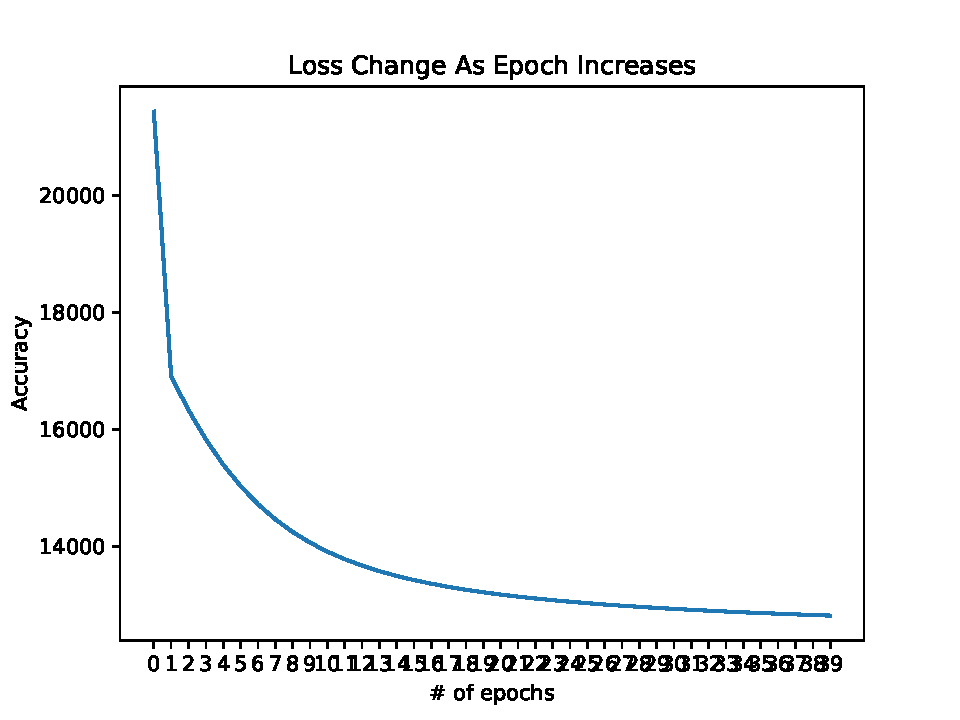
\includegraphics[scale=0.7]{figures/generated/nn_Loss_Change_As_Epoch_Increases.pdf}

    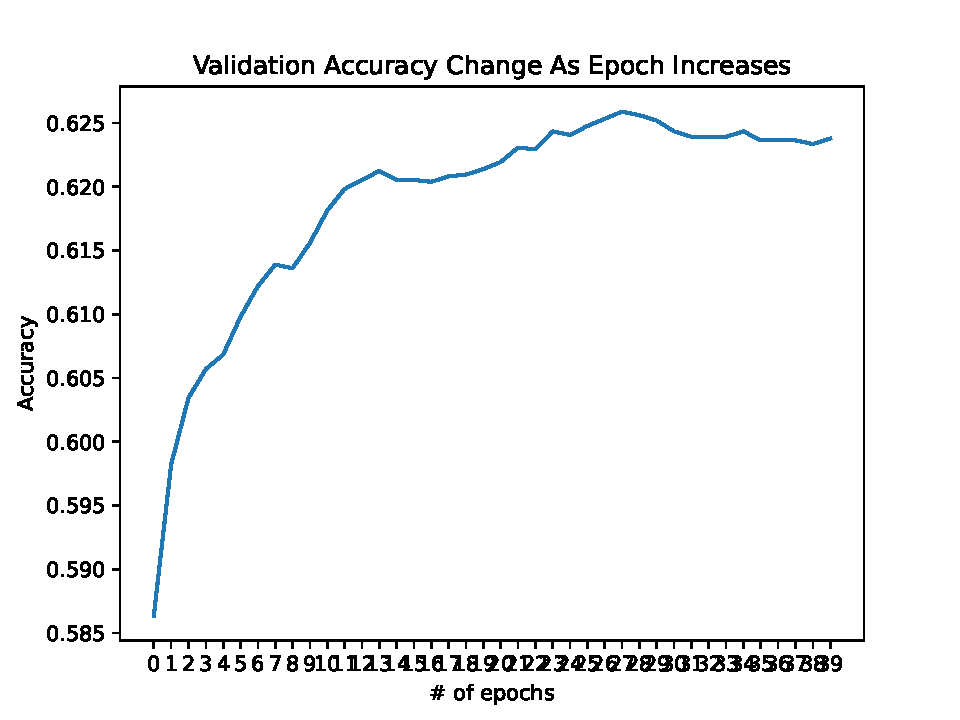
\includegraphics[scale=0.7]{figures/generated/nn_Validation_Accuracy_Change_As_Epoch_Increases.pdf}

    \subsection{Implementing $L_2$ Regularization}
    $L_2$ regularization has been implemented in the same code file as the other parts of this question (\verb|part_a/neural_network.py|).

    \begin{verbatim}
        lamb=0
        Final Validation Accuracy*    0.6858594411515665
        Final Test Accuracy*    0.6836014676827548
        lamb=0.001
        Final Validation Accuracy*    0.6869884278859724
        Final Test Accuracy*    0.6785210273779283
    \end{verbatim}

    \begin{verbatim}
        (optional extra finding):
        but with lamb=0.00025
        Final accuracy    0.6848715777589613
        Final Test Accuracy*    0.6861416878351679
    \end{verbatim}

    There are improvements on the validation accuracy, but not on the test accuracy.


    \pagebreak

    \section{Ensemble}
    Code for the ensemble is implemented in \verb|part_a/ensembly.py|. We bagged our base neural network, k-Nearest-Neighbor, and Item-Response models with their previously discussed optimal hyper parameters.

    \begin{pylabblock}[ENSEMBLE]
        import ensemble as ensemble
        ensemble.evaluate_ensemble(verbosity=1, data_path="./data")
    \end{pylabblock}

    \medskip

    Output:

    \printpythontex[verb]

    \medskip

    We selected 3 base model: kNN, item response model and autoencoder, the bootstrapping phase is done with \verb|numpy.choice|, which samples n user v from the training sparse matrix uniformly, with replacement. To accomadate at least one entree per user and to maintain user order that is required in current version of evaluation functions, we concatenated all of our samples under the original \verb|train_matrix|. We generate 3 versions of bagged train matrix then train each basemodel respectively. For final prediction, we take the average of the predictions given by the 3 trained models, if the average of the value is greater than (or equal to) $0.5$, the prediction will be $1$, otherwise, it will be $0$. Our final result on test data showed the ensemble algorithm performed better than kNN, had very close performance to neural network, and performed a bit less than item response model. To elaborate, we see that the test accuracy for the ensemble is around $69.4\%$ while the neural network's testing accuracy is around $68.6\%$, $68.4\%$ and IRT is around $70.6\%$. The average (without weighing) of the latter three is around $69.2\%$ which aligns with the first, i.e, the ensemble of the three. We believe this is because bagging may reduce variance, but will not affect the bias. It would seem that the two under-performing models, kNN and NN, dragged the accuracy down, while IRT kept it up.

    

    \pagebreak

    \part{Modifying for Higher Accuracy}
    \section{Formal Description}
    We are extending the ensemble algorithm (Part A, Question 4). The original ensemble algorithm has 3 phases: bagging (bootstrap aggregating sparse matrix) $\implies$ train (training models using the bagged matrix) $\implies$ prediction, as demonstrated in the figure below:

    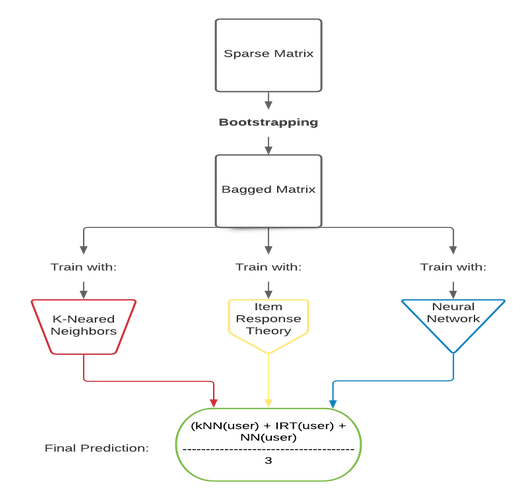
\includegraphics[scale=0.55]{figures/pb_f1.png}
    
    For this project, we gathered inspiration from the AdaBoost algorithm (Freund \& Schapire, 1999). AdaBoost is a short form of Adaptive Boosting; The algorithm is adaptive in the sense that subsequent "weak learners" are tweaked in favor of those samples misclassified by previous classifiers. The individual learners can be weak, but as long as the performance of each one is slightly better than random guessing, the final model can be proven to converge to a strong learner.
    
    As a departure from the Ensemble algorithm demonstrated in part (A), are removing kNN, modifying the bootstrapping phase (that generates a bagged matrix from the sparse matrix), and prediction phase (within the green box in figure above).

    First, our Adaboost Ensemble model does not include k-nn as a weak base model. We have omitted KNN model from our final adaboost ensemble, and instead replaced it with our previously implemented neural network model, with a differently-bagged matrix from the original neural network model. We chose this implementation because the decision surfaces of k-nn classifiers are typically too stable and any multiples of data points in the bootstrap sample do not shift the 'weight' like in many other models. [insert citation]

    The second change is instead of bootstrapping with a uniform probability distribution, we are assigning weights to each user; the weight of each user is determined by the number of questions that the previous model got wrong on this user. The initial bagging is still performed with uniform probability distribution.

    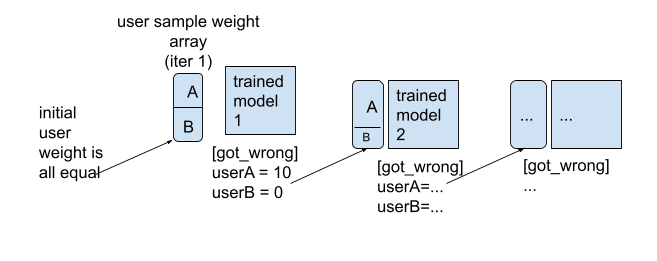
\includegraphics[scale=0.5]{figures/pb_f2.png}

    [Insert formula here]
    In the general case, After the training of a model, we obtain the number of total training entries; number of training entries that the model scored correctly {} and wrong {}, per user {}.
    We determine a training accuracy % TODO

    By focusing on the training errors the models made, we expect our model to perform better because this will reduce overfit on users that can be easily predicted, and improve underfit on users that the models struggle to predict. 

    The third change is during the prediction phase. The prediction phase, instead of generating $3$ predictions and taking the average to be the final prediction, we are assigning specific user weights to each model. These weights are for the sampled users for a bagged training set and determined by the performance of the model on said bagged training set. The model with the highest weighting of that specific user will be used for all predictions regarding that user.

    By picking a single most-suited model to predict based on which user is doing the question, we expect our model to perform better because this will eliminate the risk of bad performing models having a say on a user that they can’t predict well on.

    The original adaboost uses a general weight to predict which weight is determined by the accuracy of training data, but we believe predicting weight per specific user can further show us which model is good at predicting which user.

    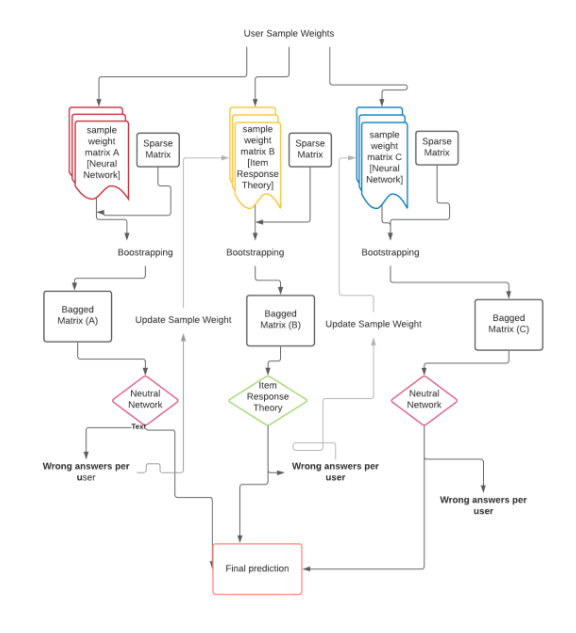
\includegraphics[scale=0.55]{figures/pb_f3.png}

    \section{Figure or Diagram}
    \section{Comparison or Demonstration}

    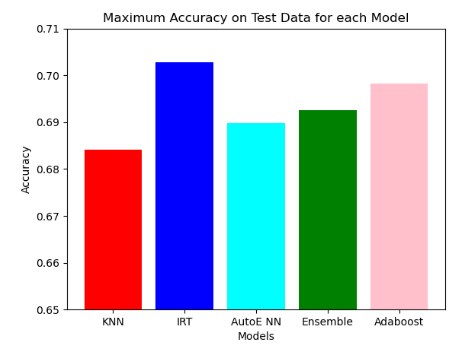
\includegraphics[scale=0.7]{figures/pb_f4.png}

    We expect our model to perform better than the original ensemble no matter what the hyperparameter is, and whether regularization is applied or not. To demonstrate this, we track the accuracy of each model for different hyperparameters, to show that the Adaboost Model outperforms the ensemble, as well as the neural network base models.

    Analysis for $k$ value:
    \begin{itemize}
        \item Modified Adaboost outperforms ensemble and neural net on most $k$, except ensembles have higher performance when $k$ is extremely large or small.
        \item An interesting finding is that the neural network model has low accuracy on $k=500$, but ensemble and modified adaboost appears to have another optimal tuning set around $k=500$. This can be further explored for future work.
    \end{itemize}

    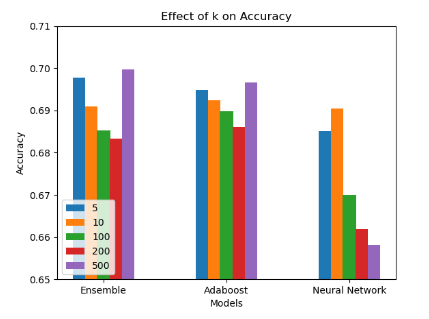
\includegraphics[scale=0.7]{figures/pb_f5.png}

    Analysis of Neural Network Epoch:
    \begin{itemize}
        \item We expected that our most suited model strategy will be resilient to overfit, this is somewhat proven, given that at epoch=100, our model outperformed the base neural model.
        \item However, the original ensemble demonstrated much more resiliency to overfit, this suggests that our final prediction determining mechanism did not meet our hypothesis, it needed to be modified.
    \end{itemize}

    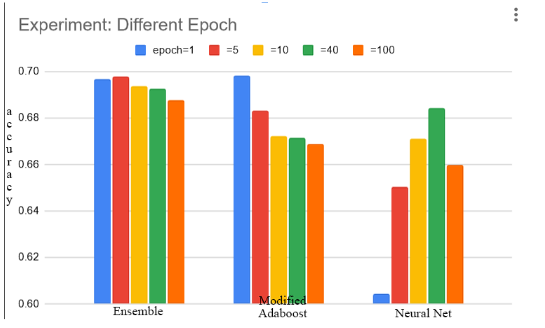
\includegraphics[scale=0.6]{figures/pb_f6.png}

    Analysis of regularization:
    \begin{itemize}
        \item 
    \end{itemize}

    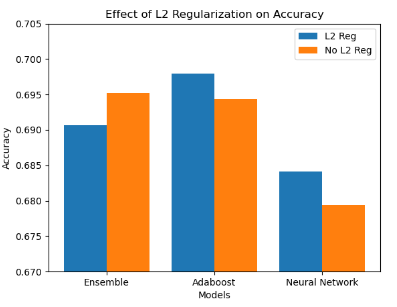
\includegraphics[scale=0.7]{figures/pb_f7.png}

    \section{Limitations}
    We will discuss some settings in which all existing methods may fail, try to guess why said methods may fail, and provide possible extensions of our Adaboost derivative that may allow for overcoming these issues.

    To start, we need to recognize that our implementation is not true adaboosting. Rather, it's a derivative however it may be considered a form of boosting, i.e, relying on weaker learners to come together and create one relatively stronger learner. In recongizing this, we can also recognize that there is an increase in sensitivity towards noise. Intuitively, this can be explained by noting that each proceeding learner in our sequence attempts to account for the errors of the previous learner. This results in magnifying potential false negatives. This may explain our low accuracy as a certain population of users we have in our training set had high prediction error rates for all three of the learning algorithms we implemented. To elaborate, these users may have had some piece of data that we did not consider, and therefore may be considered an outlier to all our algorithms. In such a case, they serve to emphasize something that (again, within the scope of our feature set), did not have a strong corellation resulting in noise, and therefore, reducing accuracy.

    To overcome this issue of having what may be considered potentially pseudo outliers, we may want to introduce more properties or features our algorithms can analyze and potentially build a model around. In other words, under the assumption that these outliers do have some common properties that serve to indicate why they may be an outlier, we can potentially model for this. A more specific solution may be to use a more elaborate neural network that has a node to account for other information on the user, such as age, time spent active (doing work), and time spend inactive, etc. This neural network may then feed into the autoencoder and the two should be optimized as one neural network.

    The previously mentioned extension is, in a sense, expanding our hypothesis space. Another thought is to reduce the hypothesis space that our data actually represents, i.e, remove the outliers that do not have the appropriate data to model them. In such a case, we may look at pre-processing the data before feeding it into our algorithm. If the issue truly was noise induced error, then this should also increase our accuracy.

\end{document}